%%% Sekce – Rezervační systém
%%%%% Wording: ⏳
%%%%% Styling: ⏳
%%%%% References: ⏳
%%% --------------------------------------------------------------
\section{Rezervační systém}
\label{sec:implementace-rezervace}
Rezervační systém je klíčovou součástí aplikace, jelikož se stará o rezervaci sedadel a vstupenek a také je zodpovědný za vypršení rezervace a jejího vymazání.
Rezervační systém je pouze jakousi integrací, nebo spíše rozšířením jádra logiky košíku.
Košík ve své podstatě pouze uchovává referenci na rezervaci ve svém stavu reprezentovanou velmi jednoduchým objektem ve tvaru rozhraní zobrazeného v ukázce kódu~\ref{lst:reservation}.

\begin{listing}[!h]
\begin{minted}{typescript}
/**
 * Reservation type
 */
export type Reservation = {
	reservationId: UUID;
	reservedUntil: Date;
};
\end{minted}
\caption{Rozhraní \texttt{Reservation}}
\label{lst:reservation}
\end{listing}

Rezervace je vytvořena v momentě, kdy je do košíku přidána první vstupenka pomocí metody \texttt{addToCartHandler()}, která je zobrazena v ukázce kódu kódu~\ref{lst:add-to-cart-handler}.

\begin{listing}[!h]
\begin{minted}[highlightlines={4-12}]{typescript}
/** add to cart handler */
const addToCartHandler = useHandler<Types.UseCart.AddToCartCb>(
	async (ticket, seat) => {
		/** create a new reservation if non-existent */
		if (!isDefined(reservation)) {
			console.log('[Cart] Creating reservation...');
			await simulatedNetworkDelay();
			/** TODO: API should be called instead */
			const reservedUntil = seat?.place === 13 ? addSeconds(new Date(), 33) : addMinutes(new Date(), 5);
			_setReservation({ reservationId: uuidv4(), reservedUntil });
			console.log('[Cart] Reservation created');
		}
		/** create a new carted ticket */
		const newCartedTicket: Types.CartedTicket = { cartedTicketId: uuidv4(), ticket, seat };
		console.log('[Cart] Adding to cart:', newCartedTicket);

		/** TODO: API should be called instead */
		await simulatedNetworkDelay();
		console.log('[Cart] Updating reserved cart');
		/** add to cart */
		_setCartedTickets([...cartedTickets, newCartedTicket]);
		return newCartedTicket.cartedTicketId;
	},
	{
		deps: [reservation, cartedTickets],
	},
);
\end{minted}
\caption{Metoda \texttt{addToCartHandler()}}
\label{lst:add-to-cart-handler}
\end{listing}

Obdobně je rezervace vymazána, když je z košíku odebrána poslední vstupenka v metodě \texttt{removeFromCartHandler()}.

%%% Podsekce – Expirace a vymazání rezervace
%%%%% Wording: ⏳
%%%%% Styling: ⏳
%%%%% References: ⏳
%%% --------------------------------------------------------------
\subsection{Expirace a vymazání rezervace}
\label{subsec:implementace-rezervace-expirace}
Více zajímavý je proces vypršení a vymazání rezervace.
To je provedeno pomocí vlastního hooku \texttt{useWaitUntil()}, který bere jako argumenty datum a \foreign{callback funkcí}\footnote{\foreign{Callback funkce} je funkce, která je předána jako argument jiné funkci a je zavolána v rámci této funkce.}.
Jednoduše čeká, dokud není dosaženo datumu, a pak zavolá tuto callback funkci, která je znázorněna v ukázce kódu~\ref{lst:clear-reservation-handler}.

\begin{listing}[!h]
\begin{minted}[highlightlines={2-5}]{typescript}
/** handle expired reservation */
useWaitUntil(reservation?.reservedUntil, async () => {
	window.alert('Reservation expired, clearing cart...');
	await clearReservationHandler.handler();
	await options.onReservationExpired();
});

/** clear reservation handler */
const clearReservationHandler = useHandler<Types.UseCart.ClearReservationCb>(
	async () => {
		console.log('[Cart] Clearing reservation...');
		await simulatedNetworkDelay();
		_setReservation(null);
		_setCartedTickets([]);
	},
	{
		deps: [reservation],
	},
);
\end{minted}
\caption{Proces expirace rezervace s metodou \texttt{clearReservationHandler()}}
\label{lst:clear-reservation-handler}
\end{listing}

Hlavní částí tohoto mechanismu je handler \texttt{clearReservationHandler()}, který opět jednoduše simuluje volání \ac{api} a poté vymaže jak rezervaci, tak obsah košík, čímž efektivně vrací košík do výchozího stavu.

%%% Podsekce – Vizualizace rezervace
%%%%% Wording: ⏳
%%%%% Styling: ⏳
%%%%% References: ⏳
%%% --------------------------------------------------------------
\subsection{Vizualizace rezervace}
\label{subsec:implementace-rezervace-vizualizace}
Rezervace je vizualizována v košíku pomocí jednoduchého odpočtu, které je uživateli zobrazeno.
Tento časovač je implementován s pomocí knihovny \texttt{react-countdown}, která poskytuje komponentu \texttt{Countdown}, která umožňuje vlastní vykreslování odpočtu.
Komponenta přijímá datum z rezervace košíku a vykresluje upozornění na rezervaci.
Toto upozornění informuje uživatele o vypršení rezervace a zbývajícím čase.
Jak je znázorněno na obrázku~\ref{fig:seating-map-reservation}, upozornění je zobrazeno v hlavičce košíku a liší se podle zbývajícího času do vypršení rezervace.

\begin{figure}[H]
	\centering
	\begin{subfigure}{0.3\textwidth}
		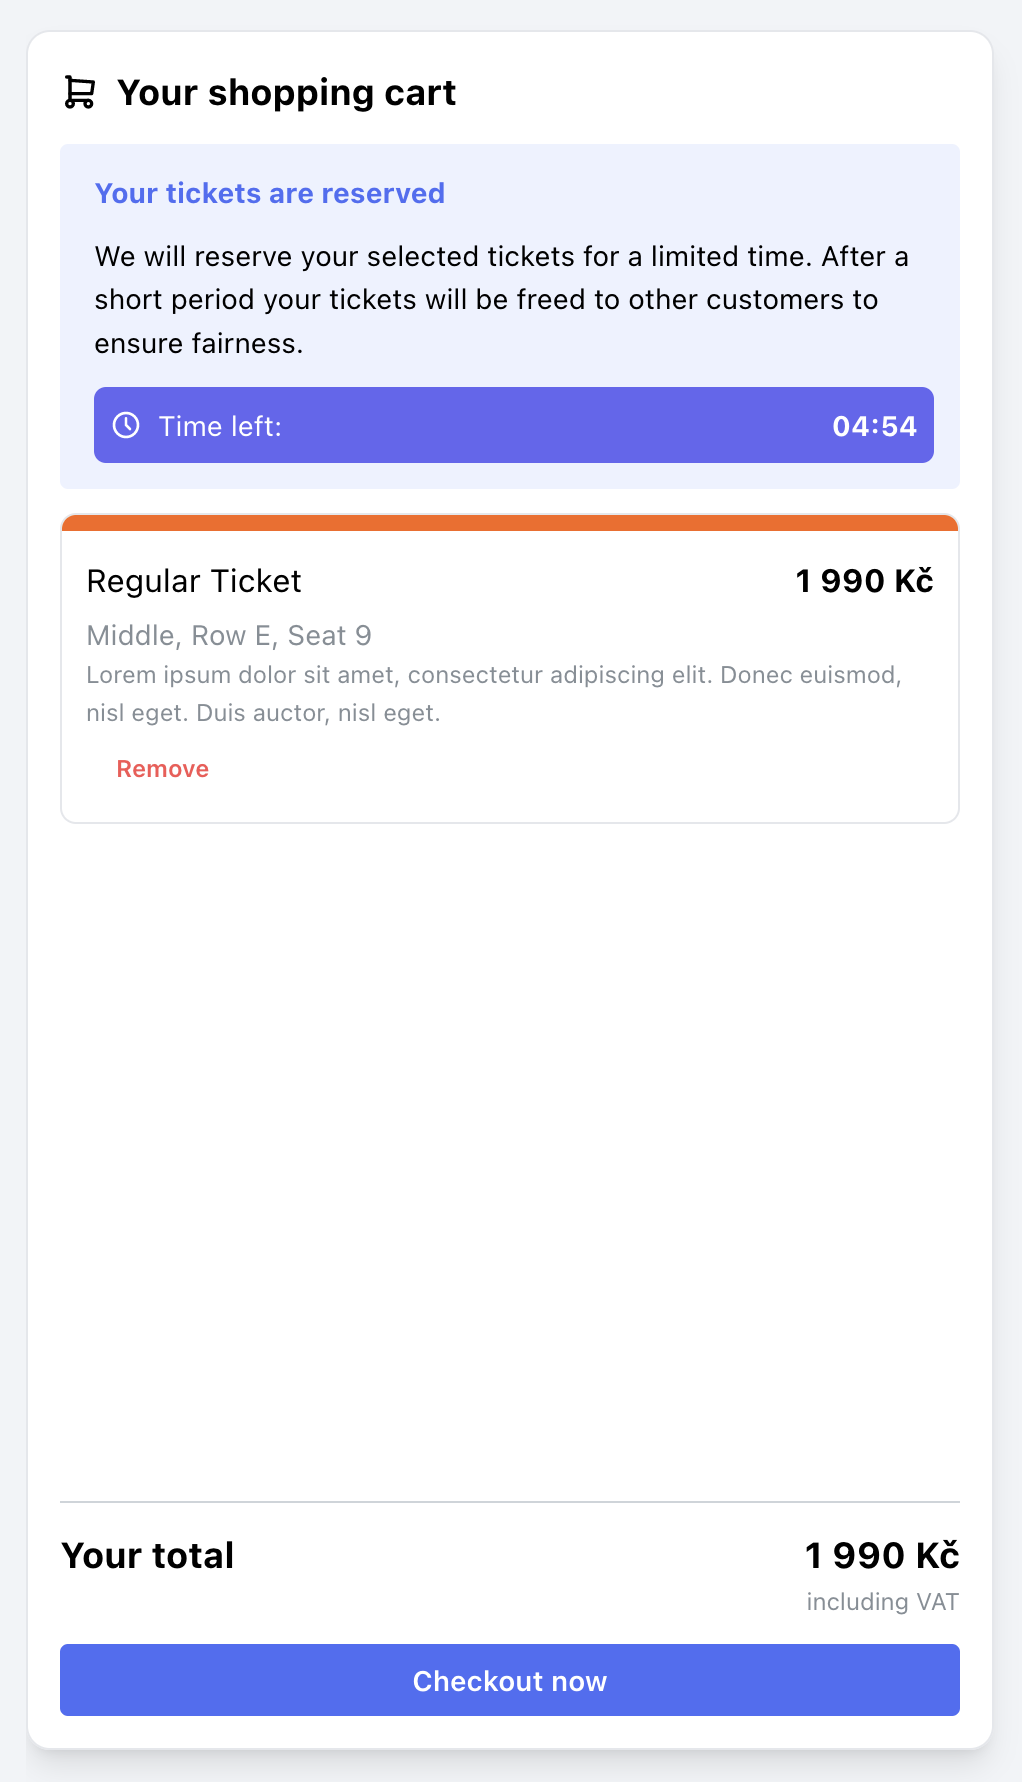
\includegraphics[width=\textwidth]{\FIGDIR/seating-map-reservation-normal}
		\caption{\geq 1 min}
		\label{fig:seating-map-reservation-normal}
	\end{subfigure}
	\hfill
	\begin{subfigure}{0.3\textwidth}
		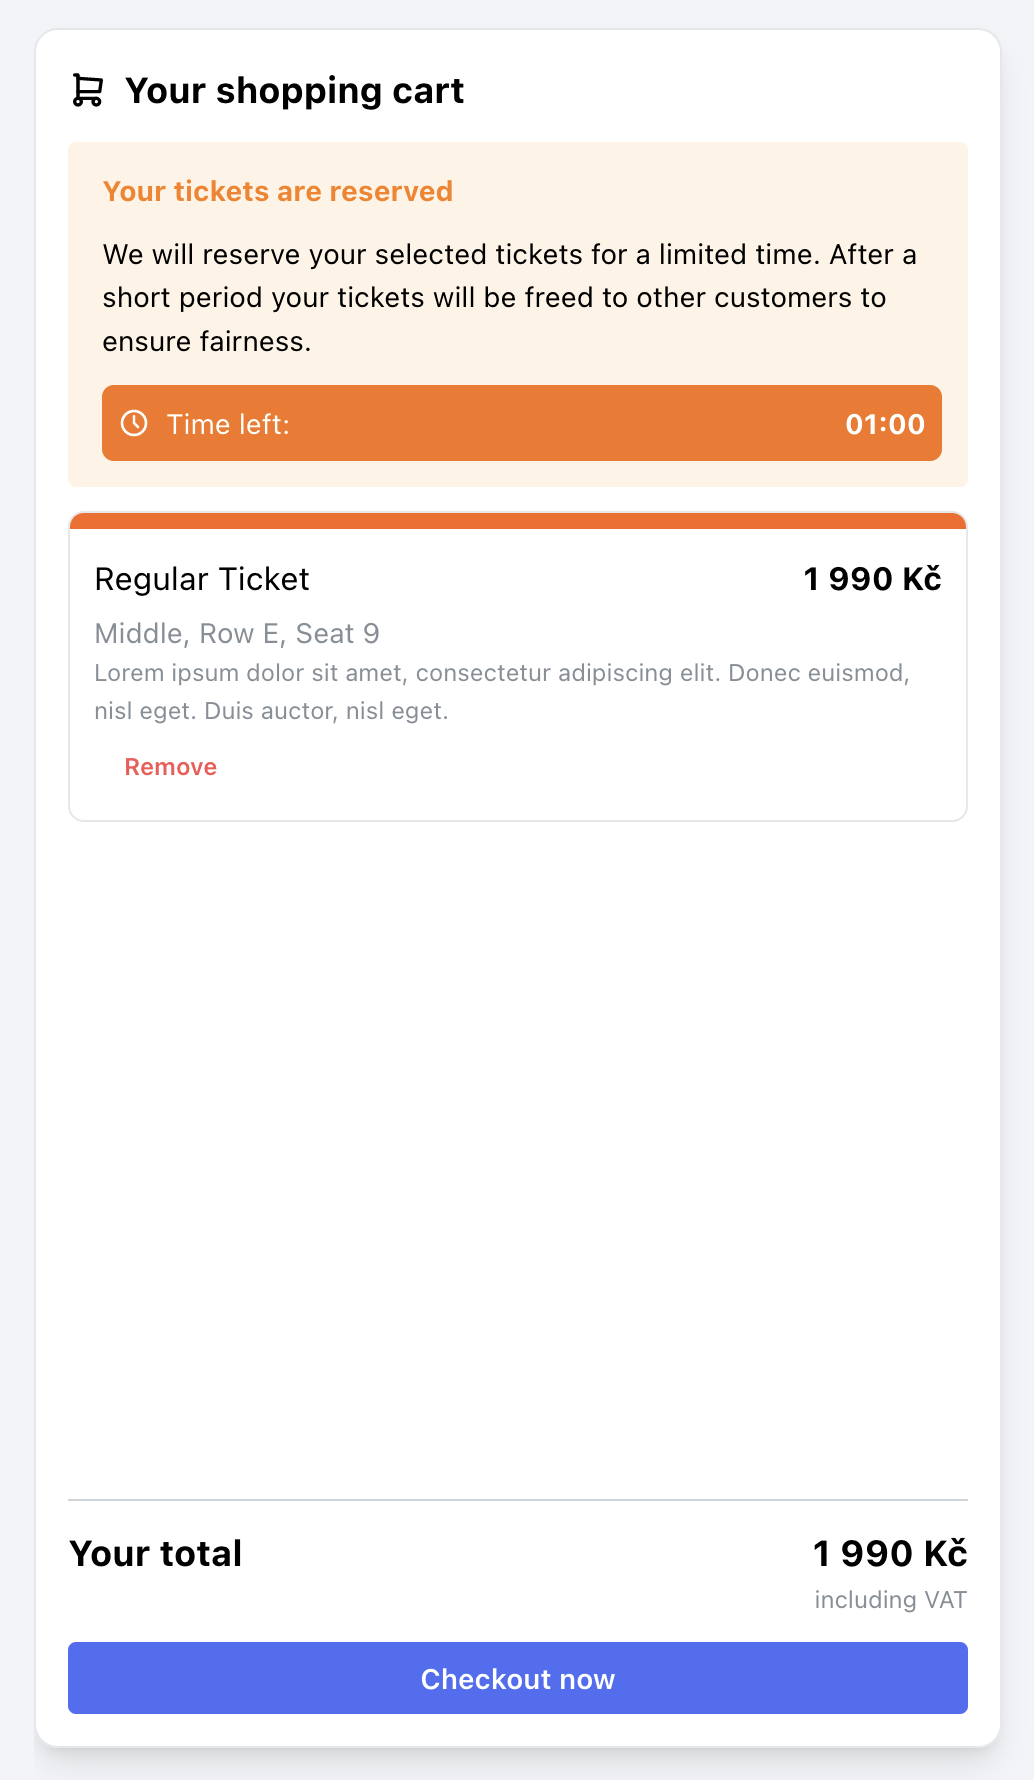
\includegraphics[width=\textwidth]{\FIGDIR/seating-map-reservation-warning}
		\caption{\textless 1 min}
		\label{fig:seating-map-reservation-warning}
	\end{subfigure}
	\hfill
	\begin{subfigure}{0.3\textwidth}
		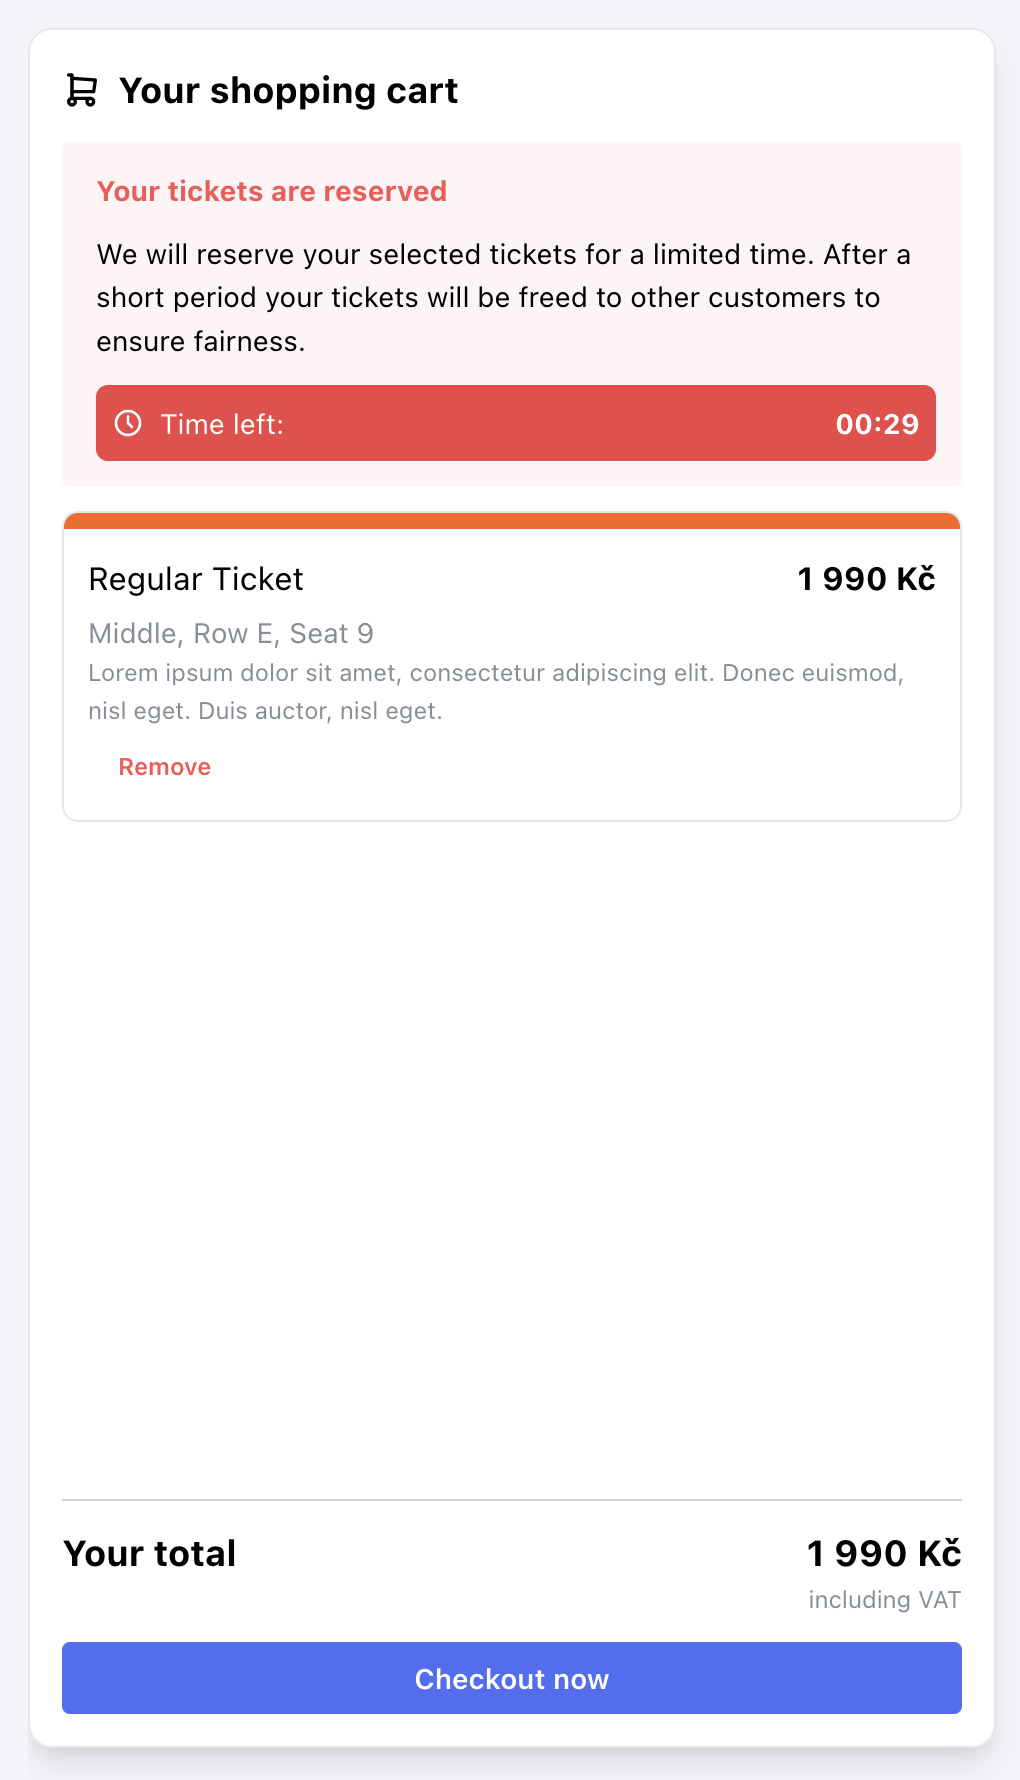
\includegraphics[width=\textwidth]{\FIGDIR/seating-map-reservation-danger}
		\caption{\leq 30 s}
		\label{fig:seating-map-reservation-danger}
	\end{subfigure}
	\caption{Upozornění na rezervaci v hlavičce košíku}
	\label{fig:seating-map-reservation}
\end{figure}

Po implementaci rezervačního systému je již košík plně funkční v rámci dané specifikace.
Další důležitou částí celé implementace je proces dokončení objednávky, který je popsán v navazující sekci~\ref{sec:implementace-checkout}.
